\chapter{Antecedentes}
	
	En este capítulo se pretende concretar el punto de partida del Proyecto. Este conocimiento base permitirá determinar en los siguiente capítulos las especificaciones del sistema a desarrollar.\\
	
	En primer lugar, se hará una breve exposición acerca del grupo de investigación AYRNA, sus miembros, sus objetivos y las actividades e investigaciones que realiza.\\
	
	Posteriormente, se analizará en profundidad los conceptos de redes neuronales y clasificación y regresión ordinal. Haciendo especial hincapié en los algoritmos previos de estudio en los que se basará el posterior algoritmo a implementar. También se hará un análisis de los parámetros de medida que se utilizarán para analizar el rendimiento de un clasificador realizando una explicación detallada de los mismos.\\
	
	Por último, se analizará el entorno y lenguaje de programación del cual se hará uso, así como del toolbox o librería que facilitará la implementación del algoritmo y optimizará computacionalmente el sistema.
	
	\section{Grupo de Investigación AYRNA}
	
		El grupo de investigación de \textit{Aprendizaje y Redes Neuronales Artificiales}, \textit{\textbf{AYRNA}} (TIC-148 de la Junta de Andalucía) fue creado en 1994 por un pequeño grupo de investigadores interesados en el campo de las Redes Neuronales Artificiales (RNAs).\\
		
		Durante los últimos años, el grupo ha diversificado sus áreas de interés, trabajando en la resolución de distintos problemas mediante técnicas de \textit{soft computing} (redes neuronales artificiales, algoritmos evolutivos y otras meta-heurísticas).\\
		
		En la actualidad, el grupo está formado por 9 investigadores doctores y 8 no doctores, siendo el investigador principal el Dr. César Hervás Martínez.\\
		
		El grupo de investigación pertenece al Departamento de Informática y Análisis Numérico de la Universidad de Córdoba y tiene su sede en la 3ª planta del edificio \textit{Albert Einstein} del Campus Universitario de Rabanales.\\
		
		Actualmente, presenta las siguiente líneas de trabajo concentradas en:
		
		\begin{itemize}
			\item Redes Neuronales Evolutivas.
			\item Modelos Híbridos de Redes de Unidades Producto (UPs), Sigmoides (Perceptrón Multicapa, MLP), Funciones de Base radial (RBFs), etc.
			\item Algoritmos Híbridos en Computación Evolutiva.
			\item Funciones Multiobjetivo para Modelos de Redes y Modelos de Computación Evolutiva.
			\item Aplicaciones en Cinética Química, Predicción de Crecimiento Microbiano, Predicción de Polen, Teledetección, etc.
			\item Programación Evolutiva.
			\item Clasificación no balanceada.
			\item Clasificación Ordinal.
			\item Aplicaciones en biomedicina, transplantes hepáticos, etc.
		\end{itemize}
	
	\section{Redes Neuronales}
		
		Una de las alternativas más utilizadas en los últimos años para la resolución de este tipo de problemas ha sido la aplicación de las llamadas redes neuronales artificiales. Ésta técnica de modelado es enormemente flexible y suele producir buenos resultados. Se fundamenta en la emulación de los sistemas nerviosos biológicos, combinando una gran cantidad de elementos simples de procesado altamente interconectado, cuya capacidad de cómputo se desarrolla mediante un proceso adaptativo de aprendizaje. Los elementos simples de procesado suelen denominarse neuronas y se agrupan en capas. Cada una de esta neuronas se encuentra interconectada con las neuronas de la capa anterior. Tradicionalmente, una red neuronal posee una capa de entrada (por la que se introducen los valores de las variables observadas), una o más capas ocultas (que realizan el procesado de dichos valores) y una capa de salida (en la que se pueden leer los valores predichos de salida). La Figura \ref{fig:rna} muestra gráficamente el aspecto de una RNA.\\
		
		\begin{figure}[h]
			\centering
			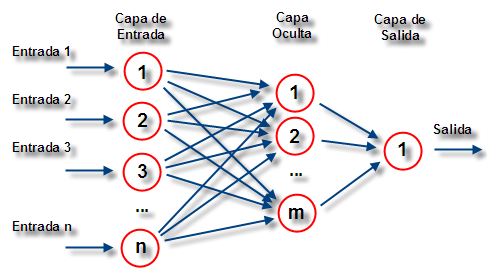
\includegraphics[scale=1]{img/rna.png}
			\caption{Red Neuronal Artificial}
			\label{fig:rna}
		\end{figure}

		Con el objetivo de lograr el aprendizaje de las redes neuronales, antes de enfrentarlas a un problema real, se requiere un proceso previo de entrenamiento que nos asegure que van a tener una buena capacidad de predicción para todos los casos, es decir, que el modelado sea eficaz.\\
		
		La Figura \ref{fig:func_rna} muestra gráficamente el funcionamiento de una RNA.\\
		
		\begin{figure}[h]
			\centering
			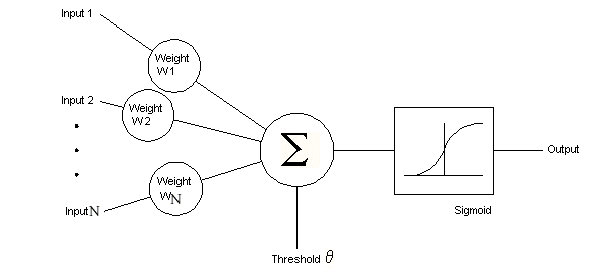
\includegraphics[scale=0.5]{img/rna_pesos.png}
			\caption{Funcionamiento de una Red Neuronal Artificial}
			\label{fig:func_rna}
		\end{figure}
		
		En 1988, el Estudio sobre Redes Neuronales realizado por DARPA\footnote{Defense Advanced Research Projects Agency (Agencia de Investigación de Proyectos Avanzados de Defensa) es una agencia del Departamento de Defensa de los Estados Unidos responsable del desarrollo de nuevas tecnologías para uso militar.} listaba varias aplicaciones con redes neuronales. Dicho estudio sirvió para que saliesen otras aplicaciones comerciales, incluyendo un pequeño reconocedor de palabras, un monitor de procesos o un clasificador de sonar.\\
		
		Las Redes Neuronales se han aplicado, además, en otros campos desde que DARPA escribió su informe. La siguiente lista contiene algunos de los campos en los que se utilizan actualmente las redes neuronales:
		
		\begin{itemize}
			\item Aeromodelismo espacial: simulación de vuelos, detección de fallos en componentes, etc.
			\item Automoción: sistemas de guía automáticos, análisis de garantías, etc.
			\item Banca: evaluación de tarjetas de crédito, etc.
			\item Defensa: búsqueda de objetivos, compresión de datos, extracción de características y supresión de ruidos, etc.
			\item Electrónica: predicción de códigos de secuencia, chip en circuitos integrados, etc.
			\item Entretenimiento: animaciones, efectos especiales, etc.
			\item Financias: análisis de uso de créditos, predicción de precios, etc.
			\item Manufactorías: control de procesos, diseño de productos, etc.
			\item Medicina: análisis de células cancerígenas, optimización de tiempos en trasplantes, etc.
			\item Robótica: control de trayectorias, controladores y manipuladores, sistemas de visión, etc.
		\end{itemize}
		
		\subsection{Regresión ordinal}
		
			La regresión ordinal (RO) permite asignar una métrica óptima a los regresores discretos de un modelo de regresión múltiple. Se trata, en síntesis, de elegir la recodificación de los predictores de acuerdo con una métrica ordinal tal, que se optimice el ajuste del modelo. De este modo, se extrae de cada regresor su mayor capacidad predictiva posible mediante una recodificación óptima de sus posibles valores en una nueva escala de naturaleza ordinal.
			
		\subsection{Algoritmo Resilient Backpropagation (RPROP)}
	
			\textit{Resilent backpropagation} (RPROP) \cite{RPROP} es una técnica de optimización robusta basada en el gradiente, que ha sido comúnmente utilizada para el entrenamiento de redes neuronales artificiales. Se basa en el uso de un valor de velocidad de avance del algoritmo para la actualización de cada parámetro del modelo.\\
	
			RPROP es una técnica ampliamente utilizada para el entrenamiento supervisado de redes neuronales artificiales tipo perceptrón multicapa, cuyo proceso de búsqueda es guiado por la primera derivada de la función $f(x)$; en este caso, $f'(x)$ es una medida de la diferencia entre la salida propuesta por la red neuronal y el valor esperado. RPROP difiere de la técnica clásica de propagación, hacia atrás, del error (o algoritmo \textit{backpropagation}) en que las derivadas parciales de la función error sólo son usadas para determinar el sentido en que deben ser corregidos los pesos de la red pero no las magnitudes de los ajustes. Los algoritmos basados en \textit{backpropagation} modifican los valores de los parámetros proporcionalmente al gradiente de la función de error, de tal forma que en regiones donde el gradiente tiende a ser plano el algoritmo avanza lentamente; esta modificación se hace con RPROP a través de un único parámetro que controla la velocidad de avance del algoritmo.\\
			
			Para comprender mejor el funcionamiento que tiene, las ecuaciones \ref{rprop1} y \ref{rprop2} muestran el funcionamiento de esta técnica:\\
			
			\begin{equation}
				\Delta w_{ij} (t) =
				\begin{cases}
					{ -\Delta p_{ij},} & \mbox{ si } \frac{ \partial E}{ \partial w_{ij}} > 0 \\
					{ +\Delta p_{ij},} & \mbox{ si } \frac{ \partial E}{ \partial w_{ij}} < 0 \\
					0, & \mbox{ si } \frac{ \partial E}{ \partial w_{ij}} = 0
				\end{cases}
				\label{rprop1}
			\end{equation}
				
			\begin{equation}
				\Delta p_{ij} (t) = 
				\begin{cases}
					{ \alpha^+ \cdot{} \Delta w_{ij}(t-1),} & \mbox{ si } \frac{ \partial E}{ \partial w_{ij}}(t-1) \cdot{} \frac{ \partial E}{ \partial w_{ij}}(t) > 0 \\
					{ \alpha^- \cdot{} \Delta w_{ij}(t-1),} & \mbox{ si } \frac{ \partial E}{ \partial w_{ij}}(t-1) \cdot{} \frac{ \partial E}{ \partial w_{ij}}(t) < 0 \\
					\Delta w_{ij}(t-1), & \mbox{ si } \frac{ \partial E}{ \partial w_{ij}}(t-1) \cdot{} \frac{ \partial E}{ \partial w_{ij}}(t) = 0
				\end{cases}
				\label{rprop2}
			\end{equation}
			
			Siendo,
			\begin{tabbing}
			\hspace{1 cm}\=\kill
			 \> $ w_ij $ los pesos o coeficientes del modelo,\\
			 \> $ t $ el instante de tiempo,\\
			 \> $ p_ij $ la actualización o cambio de los pesos,\\
			 \> $ E $ la entropía,\\
			 \> $ \alpha $ el rango de aprendizaje.
			\end{tabbing}
			
			Por otra parte, los parámetros obtenidos experimentalmente que se utilizan son,
			\begin{tabbing}
			\hspace{1 cm}\=\kill
			 \> $ \alpha^+ = 1.2, $\\ 
			 \> $ \alpha^- = 0.5, $\\ 
			 \> $ \Delta w(0) = 0.5, $\\ 
			 \> $ \Delta w(t)_{max} = 50, $\\ 
			 \> $ \Delta w(t)_{min} = 0 $
			\end{tabbing}
	
		\subsection{Algoritmo iRPROP+ (RPROP mejorado)}
	
			La variante de RPROP, iRProp+ \cite{iRPROP+}, añade un paso de vuelta atrás al algoritmo, que permite evitar los óptimos locales. La idea es que, cuando el cambio en un parámetro de la red haya producido un aumento del valor de la función de error, vuelva al estado anterior antes de producirse dicho cambio. De esta forma, se tienen las ecuaciones:\\
			
			\begin{equation}
				\Delta w_{ij} (t) = 
				\begin{cases}
					{ \alpha^+ \cdot{} \Delta w_{ij}(t-1),} & \mbox{si } \frac{ \partial E}{ \partial w_{ij}}(t-1) \cdot{} \frac{ \partial E}{ \partial w_{ij}}(t) > 0 \nonumber \\
					{ \Delta w_{ij}(t-1)-\Delta w_{ij}(t-2),} & \mbox{si } \frac{ \partial E}{ \partial w_{ij}}(t-1) \cdot{} \frac{ \partial E}{ \partial w_{ij}}(t) < 0 \nonumber \\
					& \mbox{ y } E(t) > E(t-1) \\
					\Delta w_{ij}(t-1), & \mbox{si } \frac{ \partial E}{ \partial w_{ij}}(t-1) \cdot{} \frac{ \partial E}{ \partial w_{ij}}(t) = 0 \nonumber
				\end{cases}
				\label{irprop+}
			\end{equation}
	
		\subsection{Redes Neuronales basadas en el modelo Proportional Odd Model (POM)}

			Para poder utilizar el algoritmo iRProp+ para regresión ordinal, nos vamos a basar en el modelo \textit{Proportional Odd Model} (POM) \cite{Mcc80}.\\

			Este modelo de regresión ordinal entra dentro del grupo de modelos de umbral, que se basan en suponer que la respuesta ordinal está asociada a una variable artificial medida en escala continua y modelada mediante intervalos de clase sobre la recta real. La mayoría de estos modelos se pueden representar mediante una función de rango $f(x)$ la cual transforma el vector de variables de entrada en valores de la recta real y un conjunto de umbrales $\left\{ \beta_0,\cdots,\beta_J \right\} $ que delimitan las categorías en esta recta. Diferentes formas de esta función de rango proporcionan modelos de clasificación ordinal como los que se han mencionado en el capítulo de Introducción.\\

			Bajo un punto de vista probabilístico, el modelo POM \cite{Mcc80} es el método estadístico básico de regresión ordinal y puede considerarse también como un modelo de umbral, donde $f(x)$ es una combinación lineal ponderada de las variables de entrada.\\

			La idea fundamental de este proyecto es basarnos en dicho modelo probabilístico para poder definir una red neuronal para regresión ordinal y utilizar una modificación del algoritmo iRProp+ (por su mayor eficiencia y eficacia) para optimizar los parámetros del modelo.\\
		
		\subsection{Medidas de rendimiento}
		
			Para comprobar que los resultados obtenidos después del entrenamiento y la simulación de una red neuronal artificial son buenos, es decir, que los resultados obtenidos al aplicar un algoritmo específico, se corresponden con un buen clasificador; existen unas medidas que se utilizan para poder ver la calidad o eficiencia de los resultados.\\
			
			Algunos de estas medidas se mencionarán y explicarán a continuación. Aunque existen más, estas son las más relevantes para el tema concreto que se está tratando que es la regresión ordinal mediante redes neuronales artificiales.
		
			\subsubsection{Matriz de confusión}
			
			Una matriz de confusión contiene información acerca de las clasificaciones actuales o predichas realizadas por un sistema de clasificación. El rendimiento de tales sistemas se evalúa, normalmente, usando los datos de esta matriz. La Tabla \ref{tabla_matriz_confusion} muestra la matriz de confusión para un clasificador de dos clases.\\
			
			\begin{table}[h]
				\centering
				\begin{tabular}{cc|c|c|c}
					\cline{3-4}
					& & \multicolumn{2}{|c|}{Predicho} \\ \cline{3-4}
					& & Negativo & Positivo \\ \cline{1-4}
					\multicolumn{1}{|c|}{\multirow{2}{*}{Actual}} &
					\multicolumn{1}{|c|}{Negativo} & a & b &     \\ \cline{2-4}
					\multicolumn{1}{|c|}{}                        &
					\multicolumn{1}{|c|}{Positivo} & c & d &     \\ \cline{1-4}
				\end{tabular}
				\caption{Matriz de confusión}
				\label{tabla_matriz_confusion}
			\end{table}
			
			Las entradas de la matriz de confusión tienen el siguiente significado en el contexto de nuestro estudio:

			\begin{itemize}
				\item a es el número de predicciones \textbf{correctas} en la que una instancia es negativa.
				\item b es el número de predicciones \textbf{incorrectas} en la que una instancia es positiva.
				\item c es el número de predicciones \textbf{incorrectas} en la que una instancia es negativa.
				\item d es el número de predicciones \textbf{correctas} en la que una instancia es positiva.
			\end{itemize}

			En el campo de la Inteligencia Artificial, una matriz de confusión es una herramienta de visualización usada normalmente en aprendizaje supervisado (en aprendizaje no supervisado se le suele llamar matriz de coincidencias). Uno de los beneficios de usar una matriz de confusión es, que es muy fácil ver si el sistema distingue entre las dos clases.\\
			
			Los siguientes términos son importantes para la comprensión de los valores de la matriz de confusión del ejemplo:\\

    		La precisión (AC - accuracy) es la proporción del número total de predicciones que fueron correctas. Se calcula usando la siguiente ecuación:\\

			\begin{equation}
				AC = \frac{a+d}{a+b+c+d}
				\label{AC}
			\end{equation}
			\\

		    Un verdadero positivo (TP - true possitive) es la proporción de casos positivos que se identificaron correctamente, se calcula mediante la siguiente ecuación:\\

			\begin{equation}
				TP = \frac{d}{c+d}
				\label{TP}
			\end{equation}
			\\

			Un falso positivo (FP - false possitive) es la proporción de casos negativos que se clasificaron incorrectamente como positivos, se calcula mediante la siguiente ecuación:\\

			\begin{equation}
				FP = \frac{b}{a+b}
				\label{FP}
			\end{equation}
			\\

			Un verdadero negativo (TN - true negative) se define como la proporción de casos negativos que se clasificaron correctamente, se calcula mediante la siguiente ecuación:\\

			\begin{equation}
				TN = \frac{a}{a+b}
				\label{TN}
			\end{equation}
			\\

		    Un falso negativo (FN- false negative) es la proporción de casos positivos que fueron incorrectamente clasificados como negativos, se calcula mediante la siguiente ecuación:\\

			\begin{equation}
				FN = \frac{c}{c+d}
				\label{FN}
			\end{equation}
			\\

			Por último, la proporción (P) es la proporción de los casos positivos predichos que fueron correctos, se calcula mediante la siguiente ecuación:\\

			\begin{equation}
				P = \frac{d}{b+d}
				\label{P}
			\end{equation}
			\\
		
			\subsubsection{Ratio Correctamente Clasificado (Correctly Classified Rate (CCR))}
			
			Cuando se tiene más de dos clases en el modelo se calcula la precisión o CCR, que es el número de elementos en la diagonal principal de la matriz de confusión, es decir, la suma del número de predicciones correctas en la que una instancia es negativa más el número de predicciones correctas en la que una instancia es positiva, dividido por el número total de elementos de la matriz.\\
			
			Anteriormente se ha visto como la precisión o AC, pero generalizando para este caso en concreto, se puede decir que corresponde a la siguiente ecuación:\\
			
			\begin{equation}
				CCR = \frac{\text{nº de bien clasificados}}{\text{nº total de patrones}}
				\label{CCR}
			\end{equation}
			\\
		
			\subsubsection{Error Absoluto Medio (Mean Absolute Error (MAE))}
			
			En estadística, el error absoluto medio es una cantidad usada para medir como de buenos son los pronósticos o predicciones de los resultados. El error absoluto medio (MAE) viene dado por la siguiente ecuación:
			
			\begin{equation}
				MAE = \frac{1}{n} \sum_{i=1}^n{\left |{f_i-y_i}\right |} = \sum_{i=1}^n{\left |{e_i}\right |}
				\label{MAE}
			\end{equation}
			\\
			
			Como su propio nombre indica, el error absoluto medio es una media de los errores absolutos, $ e_i = f_i-y_i $, donde $ f_i $ es la predicción e $ y_i $ es el valor verdadero. Existe una notación alternativa en la que se puede incluir frecuencias relativas como factores de peso.\\

			El error absoluto medio es una medida común de pronóstico de errores en análisis temporales de series, donde el término ``error absoluto medio" se utiliza en algunas ocasiones confundiéndolo con la definición más estandarizada de desviación media absoluta.\\

			El MAE mide la magnitud media de los errores en un conjunto de pronóstico, sin considerar su dirección. Así, se puede decir que mide la precisión para variables continuas.\\
			
			También es una medida específica para clasificación ordinal. Donde se realiza el sumatorio de los  errores cometidos por un clasificador en valor absoluto asignando una etiqueta numérica a cada clase. Para ahorrar coste computacional, el error absoluto medio también se puede calcular en base a la matriz de confusión explicada anteriormente, multiplicando ésta por una matriz de costes del estilo a la mostrada:
			
			\begin{equation}
				MP = 
					\begin{bmatrix}
						{0}&{1}&{2}&{3}\\
						{1}&{0}&{1}&{2}\\
						{2}&{1}&{0}&{1}\\
						{3}&{2}&{1}&{0}
					\end{bmatrix}
				\label{matriz_pesos}
			\end{equation}
			\\
			
			Multiplicando elemento a elemento, no de forma matricial, la matriz de confusión por esta otra matriz de pesos, resultará una matriz de errores absolutos. Dándole un peso proporcional a la distancia entre aquellos elementos mal clasificados. En este momento, haciendo el sumatorio de todos los elementos de la matriz y dividiéndolo por el número total de elementos, se obtendrá el MAE. La siguiente ecuación muestra lo explicado anteriormente:
			
			\begin{equation}
				MAE = \frac{\sum{(MC \cdot{} MP)}}{TOTAL}
				\label{matriz_mae}
			\end{equation}
			\\
			
			\subsubsection{Error Cuadrático Medio (Mean Square Error (MSE))}
			
			En estadística, el error cuadrático medio o MSE de un estimador es uno de los posibles caminos para cuantificar la diferencia entre un estimador y el valor verdadero de la cantidad que se va a estimar, es decir, es la media aritmética de los cuadrados de las desviaciones del estimador $\hat{\theta}$ respecto al valor verdadero del estadístico que se trata de estimar.\\

			Se diferencia de la varianza en que, en ésta, las desviaciones son con respecto a la media aritmética. Lógicamente, cuando el estimador sea insesgado, el error cuadrático medio será igual a la varianza.\\
			
			El MSE de un estimador con respecto al parámetro estimado $\hat{\theta}$ se define como:

			\begin{equation}
				MSE(\hat{\theta}) = E[(\hat{\theta}-\theta)^2]
				\label{estimator_mse}
			\end{equation}
			\\

			El MSE también se puede calcular sumando la varianza al cuadrado del sesgo o \textit{bias} del estimador:

			\begin{equation}
				MSE(\hat{\theta}) = Var(\hat{\theta})+\left(Bias(\hat{\theta},\theta)\right)^2
				\label{varianza_mse}
			\end{equation}
			\\
		
	\section{Matlab}
	
		MATLAB es un lenguaje de computación de alto nivel y un entorno interactivo para desarrollo de algoritmos, visualización de datos, análisis de datos y cálculo numérico. Con MATLAB, se puede resolver problemas de cálculo más rápidamente que con lenguajes de programación tradicionales, tales como C, C++ o Fortran.\\
		
		El lenguaje de MATLAB incluye operaciones vectoriales y matriciales que son fundamentales para resolver los problemas científicos y de ingeniería. Agiliza tanto el desarrollo como la ejecución.\\

		Con el lenguaje de MATLAB, se puede programar y desarrollar algoritmos más rápidamente que con los lenguajes tradicionales porque ya no hay que realizar tareas administrativas de bajo nivel, tales como declarar variables, especificar tipos de datos o asignar memoria. En muchos casos, MATLAB elimina la necesidad de bucles ``for", o condiciones explícitas ``if". Por ello, una línea de código de MATLAB generalmente reemplaza a varias líneas de código en C/C++, Fortran o JAVA.\\

		Al mismo tiempo, MATLAB ofrece todas las características de los lenguajes de programación tradicionales, que incluyen operadores aritméticos, control de flujo, estructuras de datos, tipos de datos, programación orientada a objetos (OOP) y depuración.\\
		
		MATLAB permite ejecutar comandos o grupos de comandos uno a uno, sin compilar ni enlazar, y repetir su ejecución hasta lograr la solución óptima.\\
		
		También ofrece todas las funciones gráficas necesarias para visualizar datos de ingeniería y científicos. Incluye funciones de representación de diagramas bidimensionales y tridimensionales, visualización de volumen tridimensional, herramientas para crear diagramas en forma interactiva y la posibilidad de exportar los resultadas a los formatos gráficos más conocidos. Se puede personalizar los diagramas añadiendo varios ejes, cambiando los colores de las líneas y marcadores, añadiendo anotaciones, ecuaciones LaTeX, leyendas y trazando formas.\\
		
		MATLAB es un software multiplataforma y eso facilita que cualquiera pueda hacer desarrollos en Matlab en su propio sistema operativo.
	
		\subsection{Toolbox \textit{nnet} (Neural Network Toolbox)}
		
			Neural Network Toolbox proporciona herramientas para el diseño, implementación, visualización y simulación de redes neuronales artificiales. Las redes neuronales se utilizan para aplicaciones donde el análisis formal es difícil o imposible, tales como reconocimiento de patrones o los sistemas no lineales de identificación y control. El toolbox soporta redes con conexiones hacia adelante o ``feedforward", redes de base radial, redes dinámicas, mapas auto-organizados u otros paradigmas de red probadas.\\

			Las redes neuronales se componen de elementos simples funcionando en paralelo. Estos elementos están inspirados en los  sistemas nerviosos biológicos. Al igual que en la naturaleza, las conexiones entre los elementos determinan en gran medida la función de red. Se puede entrenar una red neuronal para realizar una función en particular, mediante el ajuste de los valores de las conexiones (pesos) entre los elementos.\\

			Por lo general, las redes neuronales se ajustan o se entrenan de modo que una determinada entrada conducirá a una salida específica.
			
		\subsection{Interfaces gráficas con Matlab}
			
			Matlab proporciona la posibilidad de crear Interfaces Gráficas de Usuario (GUI\footnote{Graphical User Interface.}) de varias formas, por ejemplo, a través de librerías de interfaz externas que permiten implementarlas escritas en C/C++, JAVA y Fortran o utilizando su aplicación gráfica para la creación de interfaces o realizando la interfaz programándola directamente a través de ficheros MAT.\\
			
			Una Interfaz Gráfica de Usuario es una exposición gráfica en una o más ventanas que contiene controles, componentes de llamada, que permite al usuario realizar tareas interactivas con un sistema. El usuario de la GUI no tiene porque crear un script o escribir comandos en la línea de comandos para realizar las tareas. Ésto ayuda a los usuarios a comprender los detalles de cómo se realizan las tareas.\\
			
			Los componentes que puede incluir una GUI pueden ser tales como menús, barras de herramientas, botones de varios tipos, listas de selección, etc. Las GUIs creadas usando las herramientas de MATLAB pueden realizar cualquier tipo de computación, como por ejemplo, leer y escribir en ficheros externos, comunicarse con otras GUIs o mostrar datos como gráficos.\\
			
			Como se ha comentado antes, se podrán realizar GUIs con MATLAB de dos maneras posibles:
			
			\begin{itemize}
				\item Usando la herramienta para creación de interfaces gráficas que contiene llamada GUIDE (GUI Development Environment)\footnote{Entorno de Desarrollo para GUI. La aplicación gráfica es muy simple y se asemeja mucho a la aplicación QTCreator para creación de interfaces gráficas con C++.}.
				\item O creando los ficheros de código fuente que generarán las GUIs como funciones o scripts (a esta técnica se la denomina \textit{construcción programada de GUIs}).
			\end{itemize}
